\section{Návrh zapojení a tvorba DPS}
    Řídící jednotka je tvořena jednou speciálně navrženou DPS, která kromě samotného mikrokontroleru obsahuje také měnič napětí typu BUCK ke snížení napájecího napětí externího zdroje na hodnotu \qty{5.2}{V} (odůvodnění v~sekci~\ref{subsec:pocet-a-fce-vodicu-sbernice}). Toto napětí pak bude dále používáno pro napájení samotného mikrokontroleru řídící jednotky a zároveň vyvedeno na konektor pro připojení periferií. Blokové schéma na úrovni logických bloků v~rámci jedné DPS je na obr.~\ref{fig:ridici-jednotka-blokove-schema}, jednotlivým částem se blíže věnují další sekce. Celé schéma je k~dispozici v~příloze~\ref{priloha:schema-ridici-jednotka}.

    \begin{figure}[h!]
        \centering
        % trim=left bottom right top
        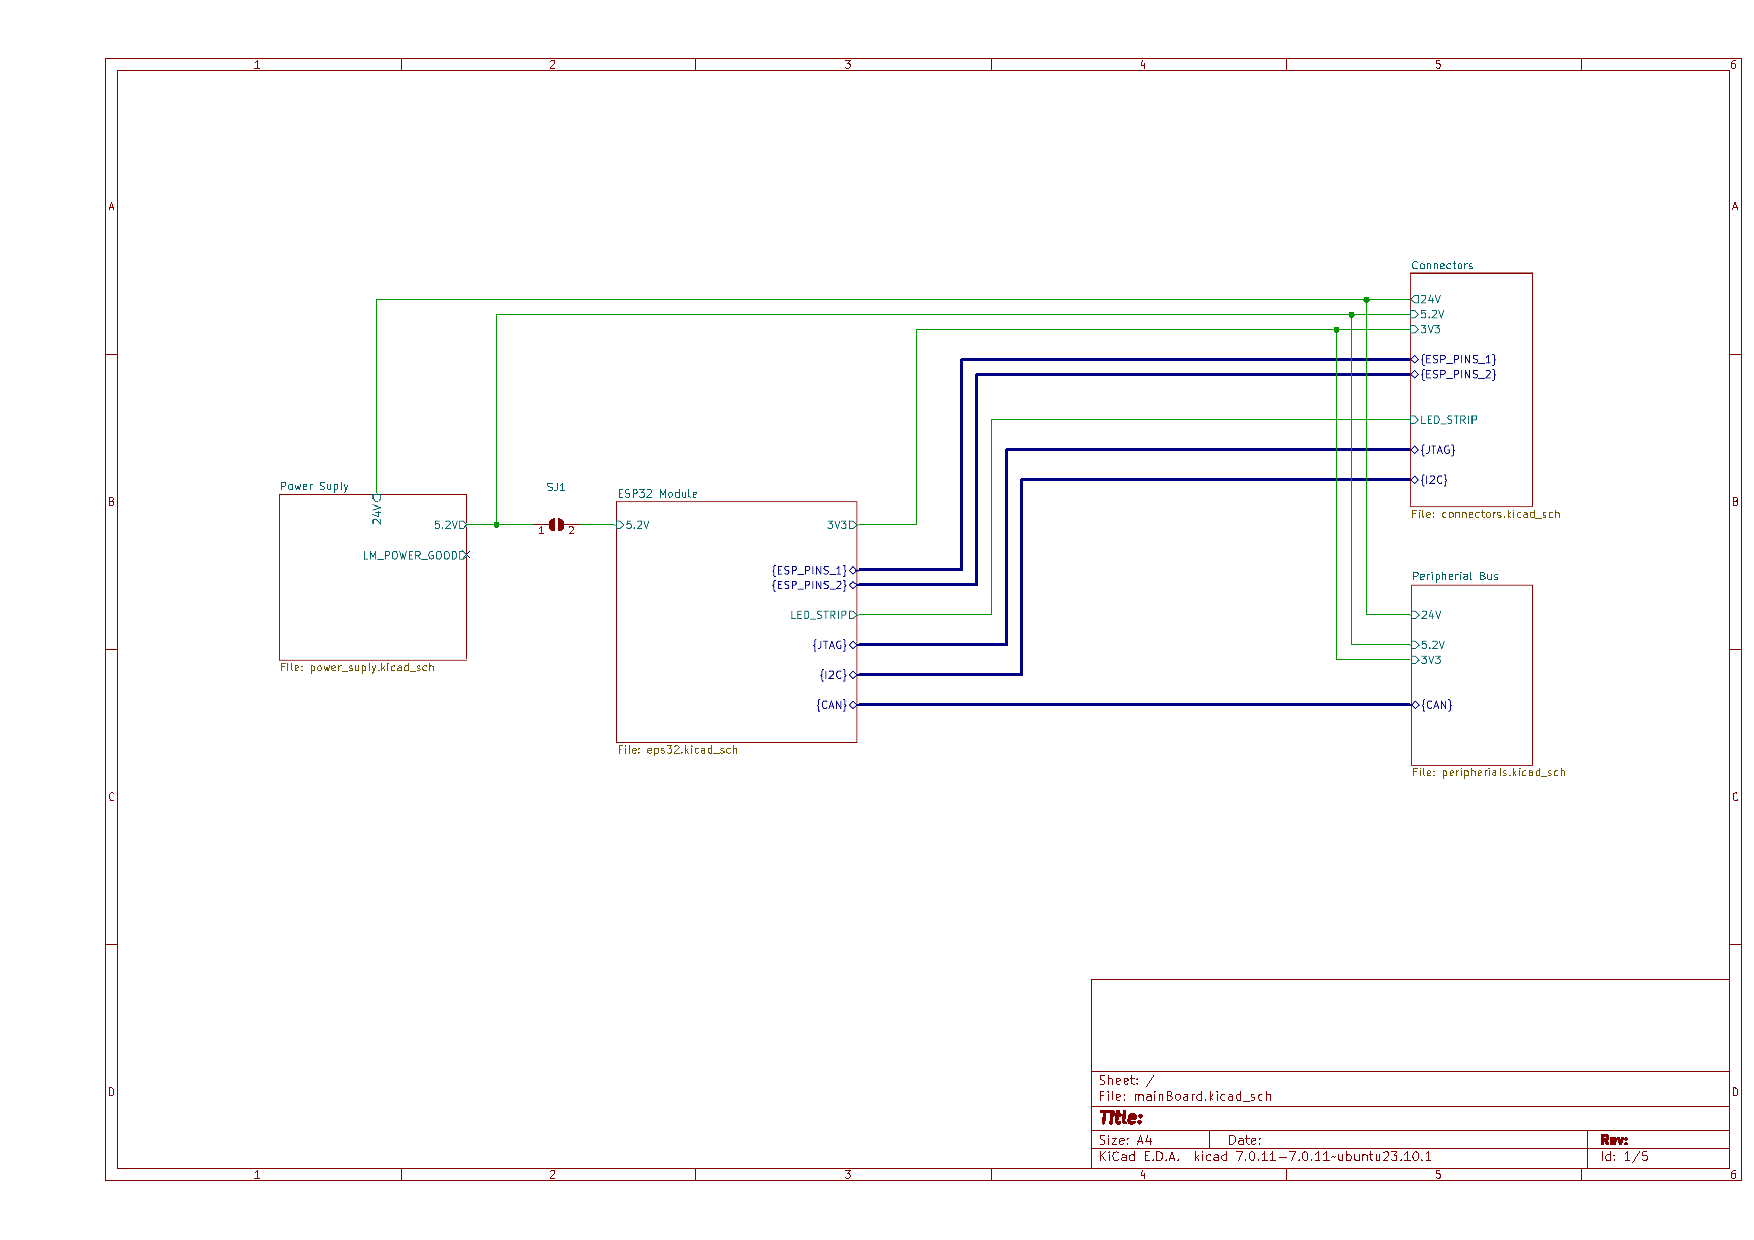
\includegraphics
        [
            width=\textwidth, 
            page=1, 
            trim=4.5cm 7.5cm 3cm 4cm, 
            clip
        ]{obrazky/exportovane/main-board-schematic.pdf}
        \caption{Blokové schéma řídící jednotky. Vytvořeno v~KiCad 7.0.}
        \label{fig:ridici-jednotka-blokove-schema}
    \end{figure}
    % TODO: jiná blokovka než z kicadu
    \subsection{Zapojení ESP32 modulu}
        Při tvorbě schématu bylo vycházeno z~dokumentace výrobce~\cite{esp32-wroom-32e-datasheet} a také ze schématů různých existujících vývojových desek. K~zajištění správné a spolehlivé funkce modulu je potřeba dodržet několik věcí. Výřez schématu obsahující potřebné doplňující obvody je na obr.~\ref{fig:ridici-jednotka-esp-obvody}.

        \begin{figure}[h!]
            \centering
            % trim=left bottom right top
            \includegraphics
            [
                width=0.9\textwidth, 
                page=2, 
                trim=2.5cm 6cm 15.5cm 1.5cm, 
                clip
            ]{obrazky/exportovane/main-board-schematic.pdf}
            \caption{Podpůrné obvody pro modul ESP32-WROOM-E. Vytvořeno v~KiCad 7.0.}
            \label{fig:ridici-jednotka-esp-obvody}
        \end{figure}

        Na napájecí pin (3V3) je třeba přivést stabilní napětí a opatřit ho blokovacími kondenzátory (C1, C3). Ke snížení napětí z~původních \qty{5,2}{V} na požadovaných \qty{3,3}{V} je použit lineární regulátor TLV76133 (U4). 
        
        Dále je potřeba přivést kladné napětí na povolovací pin (EN), z~dokumentace vyplývá, že by mělo být přivedeno až po ustálení napájecí linky. Uvedený čas nutný ke stabilizaci je roven \(t_{STBL}=\qty{50}{\micro\second}\)~\cite{esp32-datasheet}. Požadované zpoždění zajistí RC článek (R1, C2) s~časovou konstantou \(\tau\):
        \begin{equation}
            \tau=R_{1}C_{2}=\qty{10}{\kilo\ohm}\cdot \qty{1}{\micro\farad}=\qty{10}{\milli\second}
        \end{equation} 
        Jak je vidět, byla zvolena dostatečná návrhová rezerva. 

        Pro možnost resetu zařízení a vstupu do bootloaderu byla doplněna také dvě tlačítka (SW1, SW2).



    \subsection{Napájecí obvod}
        \label{sec:ridici-jendotka-napajeci-obvod}
        % \textit{TODO: schéma, výpočet hodnot součástek}
        Pro napájení celého zařízení je použit externí zdroj stejnosměrného napětí \qty{24}{V}, toto napětí je rozvedeno všem připojeným periferiím (viz sekce~\ref{subsec:pocet-a-fce-vodicu-sbernice}). Pro většinu komponent je ale nutné napětí snížit. K~tomuto účelu byl navržen DC/DC měnič typu buck s~požadovaným výstupním napětím \qty{5.2}{V}. Existuje celá řada čipů vyvinutých pro tento účel. Aplikace v~tomto zařízení je specifická svými požadavky na výstupní proud, zatímco samotná řídící jednotka nebude odebírat velký proud, není jasně dané, kolik periferí a s~jakými výkonovými požadavky uživatel k~systému připojí. Navržený měnič tak musí fungovat v~širším rozsahu proudů (řádově od desítek mA po jednotky A) a to s~co nejlepší účinností. 
        
        \begin{figure}[h!]
            \centering
            % trim=left bottom right top
            \includegraphics
            [
                width=0.9\textwidth, 
                page=3, 
                trim=5.5cm 4.5cm 4cm 2.5cm, 
                clip
            ]{obrazky/exportovane/main-board-schematic.pdf}
            \caption{Napájecí obvod řídící jednotky. Vytvořeno v~KiCad 7.0.}
            \label{fig:ridici-jednotka-napajeni}
        \end{figure}
        % TODO: nove schema dodat

        Aby bylo vyhověno zmíněným požadavkům a zachována návrhová rezerva, byl jako základ buck měniče zvolen čip LM5148~\cite{lm5148-datasheet}. Jedná se o~moderní součástku firmy Texas Instruments s~velkou výkonovou rezervou. Tento čip funguje pouze jako buck kontroler a je potřeba doplnit zapojení dvěma externími MOSFET tranzistory, většina tepelných ztrát vzniká právě na nich, čímž se sníží ohřev samotného čipu a generované teplo se lépe rozloží. Na volbě tranzistorů závisí také výsledná účinnost měniče. Při návrhu zapojení této součástky byl použit nástroj Webench Power Designer~\cite{webench-power-designer}, který podle zadaných porametrů navrhne konkrétní schéma zapojení, provede simulaci a zobrazí grafy upravené na míru podle zvolených hodnot. Tento nástroj uvádí přibližnou účinnost zapojení jako \qty{88}{\percent}. V~navrženém schématu bylo posléze provedeno několik změn, aby vše odpovídalo požadavkům uvedeným v~katalogovém listu součástky~\cite{lm5148-datasheet}. Výsledné zvolené zapojení se nachází na obr.~\ref{fig:ridici-jednotka-napajeni}. V~obrázku se nachází také odkazy ke konkrétním kapitolám katalogového listu relevantních k~volbě hodnot vybraných součástek. 

        TODO: výpočty 

    \subsection{Deska plošných spojů}
        Ačkoliv se jedná o relativně jednoduchou DPS, je potřeba při návrhu dbát jistých pravidel a doporučení 
        % sem patří zmínit ESP umístění modulu, konektory, stacup desky, buck měnič

   

    \section{Konektivita}
    \label{subsec:pocet-a-fce-vodicu-sbernice}
    Z~hlediska datové komunikace jsou zapotřebí dva vodiče (TX a RX), kromě toho je ale nutné periferiím dodat napájení. Většina periferií by měla být v~principu dosti jednoduchá a energeticky nenáročná zařízení, typicky obsahující mikrokontroler pracující s~napětím 3,3 nebo \qty{5}{V} s~jedním nebo několika málo připojenými senzory. Pro jejich napájení postačí další dva vodiče, jeden zemní, společný i pro datové vodiče, a druhý s~napětím \qty{5.2}{V}. Periferie musí být navrženy tak, aby je drobné změny této hodnoty neovlivnily. V~případě několika periferí zapojených za sebe bude na delším vedení zákonitě docházet k~poklesu napětí, proto byla zvolena návrhová rezerva \qty{0.2}{V}, která na základě praktického testu bude možná v~budoucnu ještě navýšena. Každá periferie musí obsahovat vlastní regulátor, kterým si pro svůj provoz vytvoří potřebné stabilní napětí 5 nebo \qty{3,3}{V}. 
    \begin{table}[h!]
        \centering
        \caption{Přiřazení vodičů pro konektor D-sub.}
        \label{tab:sbernice-popis-vodicu}
        \begin{tabular}{|l|l|l|l|}
            \hline
            \textbf{Č.} & \textbf{Zkratka} & \textbf{Popis} & \textbf{Napětí} \\
            \hline\hline
            2, 7 & 24V & Napájení z~externího zdroje, pro náročné periferie & \qty{24}{V} \\
            \hline
            1, 5, 6, 9 & GND & Společná zem & \qty{0}{V}\\
            \hline
            8 & 5V & Napájení pro MCU periferií & \qty{5.2}{V}\\
            \hline
            3 & CANH & Kladný vodič diferenční datové linky & 0 až \qty{3.3}{V}\\
            \hline
            4 & CANL & Záporný vodič diferenční datové linky & 0 až \qty{3.3}{V}\\
            \hline
        \end{tabular}
    \end{table}

    Některé periferie mohou mít vyšší výkonové nároky a navržené nízkonapěťové napájení by jim nemuselo stačit, zároveň by vysokým odběrem proudu klesala stabilita celé sběrnice. Pro tyto periferie je proto potřeba přivést další napájecí větev, opět o~dvou vodičích. Krom zemního vodiče přivedeme napájení \qty{24}{V}, které pochází přímo z~externího zdroje v~hlavním šasi zařízení. Daná periferie pak musí obsahovat vlastní měnič, kterým si vytvoří napětí o~potřebné velikosti. 

    Všechny zmíněné vodiče jsou pro lepší přehlednost shrnuty v~tab.~\ref{tab:sbernice-popis-vodicu}.


% TODO: toto jsem tu jen hodil, at vidim, že to existuje
    Dále bylo nutné vybrat vratnou pojistku s~vhodnými parametry. Maximální provozní proud, který může po sběrnici téct je limitovaný sériovým odporem a pro zvolenou hodnotu \qty{100}{\ohm} odpovídá \(I_{max} =\qty{33}{mA}\), této hodnoty ale nikdy nedosáhne stabilně nýbrž pouze na krátký čas při změně mezi logickou nulou a jedničkou. Byla proto zvolena pojistka s~hodnotou limitního proudu \(I_{trip} =\qty{60}{mA}\) a běžného provozního proudu \(I_{hold} =\qty{20}{mA}\). 

\section{Konektor - TODO: pryč}
    Hlavní šasi bude disponovat dvěma konektory typu samice. Každá periferie bude mít napevno připevněn kabel zakončený konektorem typu samce a na své krabičce pak opět jeden konektor typu samice. Periferie tedy bude možné připojit buďto přímo do jednoho ze slotů hlavního šasi anebo do série s~některou jinou již připojenou periferií. 

    V~principu lze zvolit jakýkoliv typ konektoru disponující alespoň šesti piny, musí však být možné konektor pohodlně použít jak na zakončení kabelu, tak i jako montovaný do panelu, např. na hlavním šasi. Volba konkrétního typu dosud nebyla provedena.


            